%% abtex2-modelo-trabalho-academico.tex, v-1.9.6 laurocesar
%% Copyright 2012-2016 by abnTeX2 group at http://www.abntex.net.br/ 
%%
%% This work may be distributed and/or modified under the
%% conditions of the LaTeX Project Public License, either version 1.3
%% of this license or (at your option) any later version.
%% The latest version of this license is in
%%   http://www.latex-project.org/lppl.txt
%% and version 1.3 or later is part of all distributions of LaTeX
%% version 2005/12/01 or later.
%%
%% This work has the LPPL maintenance status `maintained'.
%% 
%% The Current Maintainer of this work is the abnTeX2 team, led
%% by Lauro César Araujo. Further information are available on 
%% http://www.abntex.net.br/
%%
%% This work consists of the files abntex2-modelo-trabalho-academico.tex,
%% abntex2-modelo-include-comandos and abntex2-modelo-references.bib
%%

% ------------------------------------------------------------------------
% ------------------------------------------------------------------------
% abnTeX2: Modelo de Trabalho Academico (tese de doutorado, dissertacao de
% mestrado e trabalhos monograficos em geral) em conformidade com 
% ABNT NBR 14724:2011: Informacao e documentacao - Trabalhos academicos -
% Apresentacao
% ------------------------------------------------------------------------
% ------------------------------------------------------------------------


\documentclass[
  10.5pt,				  % tamanho da fonte
	openright,			% capítulos começam em pág ímpar (insere página vazia caso preciso)
	twoside,			  % para impressão em recto e verso. Oposto a oneside  
  a5paper,
  chapter=TITLE,	% títulos de capítulos convertidos em letras maiúsculas
	section=TITLE,	% títulos de seções convertidos em letras maiúsculas
  hyphens,        % faz a quebra de linhas em URLs muito longas
	% -- opções do pacote babel --
	english,        % idioma adicional para hifenização
	brazil          % o último idioma é o principal do documento
]{abntex2}

% ---
% Pacotes básicos 
% ---
\usepackage{lmodern}          % Usa a fonte Latin Modern			
\usepackage[T1]{fontenc}      % Selecao de codigos de fonte.
\usepackage[utf8]{inputenc}	  % Codificacao do documento (conversão automática dos acentos)
\usepackage{lastpage}         % Usado pela Ficha catalográfica
\usepackage{indentfirst}      % Indenta o primeiro parágrafo de cada seção.
\usepackage{color}				    % Controle das cores
\usepackage{graphicx}			    % Inclusão de gráficos
\usepackage{microtype} 			  % Para melhorias de justificação
\usepackage[final]{pdfpages}

%\usepackage{multirow}         % Permite a mesclagem de linhas em tabelas
%\usepackage{adjustbox}        % Permite o escalonamento do conteúdo que não cabe em uma página
%\usepackage{tabularx}         % Impede o overflow de tabelas. 
%\usepackage{rotating}         % Rotaciona tabelas.
%\usepackage{placeins}         % Permite usar \FloatBarrier

% ---

% ---
% Pacotes adicionais, usados apenas no âmbito do Modelo Canônico do abnteX2
% ---
\usepackage{lipsum}				% para geração de dummy text
%\usepackage{cmap}
% ---

% ---
% Lista de símbolos e acrônimos
% ---
%\usepackage{abntex2glossaries}  % Deve ser incluído antes de abntex2cite

% ---
% Pacotes de citações
% ---
\usepackage[brazilian,hyperpageref]{backref} % Paginas com as citações na bibl
%\usepackage[alf]{abntex2cite}	              % Citações utilizando o padrão autor-data de chamadas
\usepackage[num,overcite]{abntex2cite}       % Citações utilizando o padrão numérico de chamadas
\citebrackets()


% --- 
% CONFIGURAÇÕES DE PACOTES
% --- 

% ---
% Configurações do pacote backref
% Usado sem a opção hyperpageref de backref
\renewcommand{\backrefpagesname}{Citado na(s) página(s):~}
% Texto padrão antes do número das páginas
\renewcommand{\backref}{}
% Define os textos da citação
\renewcommand*{\backrefalt}[4]{
	\ifcase #1 %
		Nenhuma citação no texto.%
	\or
		Citado na página #2.%
	\else
		Citado #1 vezes nas páginas #2.%
	\fi}%
% ---

% ---
% Correção das margens
% ---
\setlrmarginsandblock{2.5cm}{1.5cm}{*}
\setulmarginsandblock{2.0cm}{1.5cm}{*}
\checkandfixthelayout
% ---
% Correção das fontes das seções
% ---
\renewcommand{\ABNTEXchapterfont}{\fontfamily{lm}\fontseries{b}\selectfont}
\renewcommand{\ABNTEXchapterfontsize}{\normalsize}
\renewcommand{\ABNTEXsectionfont}{\ABNTEXchapterfont}
\renewcommand{\ABNTEXsectionfontsize}{\normalsize}
\renewcommand{\ABNTEXsubsectionfont}{\ABNTEXchapterfont}
\renewcommand{\ABNTEXsubsectionfontsize}{\normalsize}
\renewcommand{\ABNTEXsubsubsectionfont}{\ABNTEXchapterfont}
\renewcommand{\ABNTEXsubsubsectionfontsize}{\normalsize}
% ---
% Correção do espaçamento no primeiro parágrafo
% ---
\setlength\afterchapskip{\lineskip}
% ---
% Caminho para as imagens
% ---
\graphicspath{{./img/}}

% ----------------------------------------------------------
% PREÂMBULO
% ----------------------------------------------------------

\titulo{Atualização Tecnológica do Formulário de Inscrição do Processo Seletivo da Pós-Graduação da UFSC}
\autor{Makhles Reuter Lange}
\data{\today}
%\instituicao{Universidade Federal de Santa Catarina}
\instituicao{%
  Universidade Federal de Santa Catarina - UFSC
  \par
  Ciência da Computação}
\local{Florianópolis}
\tipotrabalho{Exemplo para referência futura}
\orientador{Andréia Alves dos Santos Schwaab}
\coorientador{Leandro José Komosinski}
\tipotrabalho{Trabalho de Conclusão de Curso}
\preambulo{Trabalho de Conclusão de Curso submetido ao Curso de Ciências da Computação da Universidade Federal de Santa Catarina para a obtenção do grau de Bacherel em Ciências da Computação.}

% ---
% Configurações de aparência do PDF final

% alterando o aspecto da cor azul
\definecolor{blue}{RGB}{41,5,195}

% informações do PDF
\makeatletter
\hypersetup{
     	%pagebackref=true,
		pdftitle={\@title}, 
		pdfauthor={\@author},
    	pdfsubject={\imprimirpreambulo},
	    pdfcreator={TeXmaker},
		pdfkeywords={tcc}{latex}{primefaces}{java}{jsf}{trabalho acadêmico}, 
		colorlinks=true,       		% false: boxed links; true: colored links
    	linkcolor=blue,          	% color of internal links
    	citecolor=blue,        		% color of links to bibliography
    	filecolor=magenta,      		% color of file links
		urlcolor=blue,
		bookmarksdepth=4
}
\makeatother
% --- 

% --- 
% Espaçamentos entre linhas e parágrafos 
% --- 

% O tamanho do parágrafo é dado por:
\setlength{\parindent}{1.0cm}

% Controle do espaçamento entre um parágrafo e outro:
\setlength{\parskip}{0.2cm}  % tente também \onelineskip

\begin{document}

% Seleciona o idioma do documento (conforme pacotes do babel)
%\selectlanguage{english}
\selectlanguage{brazil}

% Retira espaço extra obsoleto entre as frases.
\frenchspacing


% ----------------------------------------------------------
% ELEMENTOS PRÉ-TEXTUAIS
% ----------------------------------------------------------
\pretextual%
% ---
% Capa
% ---
\imprimircapa%
% ---
% Folha de rosto
% (o * indica que haverá a ficha bibliográfica)
% ---
\imprimirfolhaderosto*%
% ---
\clearpage
%\imprimirfichacatalografica%
%\clearpage

% ----------------------------------------------------------
% FOLHA DE APROVAÇÃO
% ----------------------------------------------------------

% Isto é um exemplo de Folha de aprovação, elemento obrigatório da NBR
% 14724/2011 (seção 4.2.1.3). Você pode utilizar este modelo até a aprovação
% do trabalho. Após isso, substitua todo o conteúdo deste arquivo por uma
% imagem da página assinada pela banca com o comando abaixo:
%
%\includepdf{folhadeaprovacaoassinada.pdf}
%
\begin{folhadeaprovacao}

  \begin{center}
    {\ABNTEXchapterfont\large\imprimirautor}

    \vspace*{\fill}\vspace*{\fill}
    \begin{center}
      \ABNTEXchapterfont\bfseries\Large\imprimirtitulo
    \end{center}
    \vspace*{\fill}
    
    \hspace{.45\textwidth}
    \begin{minipage}{.5\textwidth}
        \imprimirpreambulo
    \end{minipage}%
    \vspace*{\fill}
   \end{center}
        
   Trabalho aprovado. \imprimirlocal, \imprimirdata:

   \assinatura{\textbf{\imprimirorientador} \\ Orientador} 
   \assinatura{\textbf{\imprimircoorientador} \\ Coorientador}
   \assinatura{\textbf{Beatriz Wilges} \\ Convidado 1}
   \assinatura{\textbf{Verônica de Souza de Melo} \\ Convidado 2}

   \begin{comment}
  \begin{center}
    \vspace*{0.5cm}
    {\large\imprimirlocal}
    \par
    {\large\imprimirdata}
    \vspace*{1cm}
  \end{center}
  \end{comment}
\end{folhadeaprovacao}


% ----------------------------------------------------------
% RESUMOS
% ----------------------------------------------------------

\begin{resumo}
Texto do resumo.
\vspace{\onelineskip} \\
\noindent \textbf{Palavras-chave:} Formulário de Inscrição; Processo Seletivo; JavaServer Faces; Primefaces;
\end{resumo}
% ---
\begin{resumo}[Abstract]
\begin{otherlanguage*}{english}
The abstract.
\vspace{\onelineskip} \\
\noindent \textbf{Keywords:} Application Form; Selective Process; JavaServer Faces; Primefaces;
\end{otherlanguage*}
\end{resumo}


% ---
% Lista de ilustrações
% ---
%\pdfbookmark[0]{\listfigurename}{lof}
%\listoffigures*
%\cleardoublepage
% ---

% ---
% Lista de tabelas
% ---
%\pdfbookmark[0]{\listtablename}{lot}
%\listoftables*
%\cleardoublepage
% ---

% ---
% Lista de abreviaturas e siglas
% ---
\begin{siglas}
  \item[Java EE] Java Enterprise Edition
  \item[JSF]     JavaServer Faces
  \item[JPA]     Java Persistence API
  \item[SeTIC]   Superintendência de Governança Eletrônica e Tecnologia da Informação e Comunicação
\end{siglas}



% ----------------------------------------------------------
% SUMÁRIO
% ----------------------------------------------------------
\pdfbookmark[0]{\contentsname}{toc}
\tableofcontents*
\cleardoublepage
% ---



% ----------------------------------------------------------
% ELEMENTOS TEXTUAIS
% ----------------------------------------------------------
\textual%




\chapter{Introdução}
% ----------------------------------------------------------

% ---
\section{Cenário Atual}
% ---

O acesso aos cursos de Pós-Graduação da UFSC é feito através de processos seletivos. A inscrição nesses processos seletivos é feita, atualmente, de forma desorganizada: existe um sistema provisório \footnote{Vide \href{}{http://www.capg.homologacao.ufsc.br/inscricao} }, com poucas funcionalidades, que está sendo utilizado por secretarias de alguns cursos; outras utilizam o seu próprio formulário de inscrição online, enquanto que algumas não utilizam nenhum sistema de inscrição propriamente dito, restringindo-se ao uso de formulários de inscrição manuais.

O uso desses diversos sistemas de inscrição, com suas funcionalidades e interfaces distintas, acarreta em diversos problemas, tais como:

\begin{itemize}
  \item Não-reutilização do código.
  \item Falta de padronização dos requisitos e tecnologias utilizadas.
  \item Autenticação de forma não-centralizada, o que além de ser uma vulnerabilidade em termos de segurança, implica em duplicação de código.
  \item Difícil manutenibilidade;
  \item Difícil obtenção de estatísticas relacionadas aos candidatos.
\end{itemize}

% ---
\section{SeTIC}
% ---


% ---
\section{Objetivos}
% ---

% ---
\subsection{Objetivo Geral}
% ---
O objetivo principal deste Trabalho de Conclusão é desenvolver um sistema para a inscrição de candidatos nos processos seletivos dos diversos programas de Pós-Graduação da UFSC, utilizando o sistema provisório que está em uso como base.

% ---
\subsection{Objetivos Específicos}
% ---
\begin{itemize}
  \item Implementação do Módulo de Inscrição.
  \item Implementação do Módulo Administrativo.
  \item Elaboração do TCC.
\end{itemize}

% ---
\section{Resultados Esperados}
% ---
\begin{itemize}
  \item Módulo do Formulário de Inscrição.
  \item Módulo Administrativo do Processo de Inscrição.
  \item Elaboração do TCC.
\end{itemize}



\chapter{Fundamentação Teórica}
% ----------------------------------------------------------

% ---
\section{Aplicações Web}
% ---


% ---
\section{Plataforma Java, Edição Empresarial}
% ---

As \textbf{aplicações empresariais} têm o propósito de fornecer a \emph{lógica do negócio} de uma empresa. O seu gerenciamento é feito de forma centralizada e é comum a sua interação com outros softwares empresariais. A plataforma Java, Edição Empresarial (Java EE), é um conjunto de tecnologias Java que são utilizadas para o desenvolvimento de aplicações empresariais. O objetivo da plataforma é fornecer aos desenvolvedores um conjunto de especificações / APIs que permitam a diminuição do tempo de desenvolvimento, a redução da complexidade e o aumento do desempenho de aplicações empresariais\cite{javaee7}. Tais especificações são \emph{contratos} que são implementados por diversos fornecedores, \emph{e.g.}, GlassFish, Oracle WebLogic, Apache TomEE, etc.

Segundo o modelo Java EE, as aplicações são distribuídas em multi-camadas (\emph{tiered design})\footnote{Os termos \emph{tier} e \emph{layer} são ambos traduzidos para o português como ``camada''. No entanto, uma \emph{tier} representa uma unidade física, na qual um código ou processo é executado. Uma \emph{layer}, por sua vez, representa uma unidade lógica, responsável pela organização lógica do código através da abstração dos dados. Diversas \emph{layers} podem existir em computadores diferentes, ou em processos diferentes em um único computador, ou ainda em um único processo em um único computador.\cite{lhotka}}. Define-se, desta forma, responsabilidades distintas para as diferentes partes do sistema, \emph{i.e.}, para os diferentes componentes que compõem uma aplicação Java EE.

\begin{figure}[!ht]
  \caption{\label{fig:multitiered_app}Diversas camadas de uma aplicação multi-camadas.}
  \begin{center}
    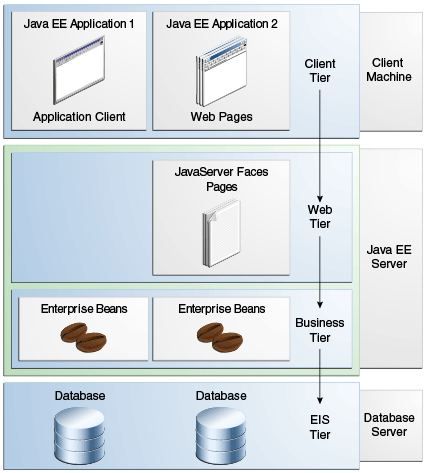
\includegraphics[width=0.75\textwidth]{multitiered_applications.png}
  \end{center}
  \fonte{adaptado de \citetext{javaee7}}
\end{figure}


% ---
\subsection{JavaServer Faces}
% ---
Apenas testando:

\begin{table}[!htb]
  \IBGEtab{%
    \caption{Um Exemplo de tabela alinhada que pode ser longa ou curta, conforme padrão IBGE.}%
    \label{tabela-ibge}
  }{%
    \begin{tabular}{ccc}
      \toprule
      Nome & Nascimento & Documento \\
      \midrule \midrule
      Maria da Silva & 11/11/1111 & 111.111.111-11 \\
      \bottomrule
    \end{tabular}%
  }{%
    \fonte{Produzido pelos autores}%
    \nota{Esta éuma nota, que diz que os dados são baseados na regressão linear.}%
    \nota[Anotações]{Uma anotação adicional, seguida de várias outras.}%
  }
\end{table}


% ---
\subsection{Facelets}
% ---

% ---
\subsection{Primefaces}
% ---

% ---
\subsection{Java Persistence API}
% ---

% ---
\subsection{Hibernate}
% ---

% ---
\subsection{Spring}
% ---



\chapter{Análise e Projeto}
% ----------------------------------------------------------

% ---
\section{Módulo do Formulário de Inscrição}
% ---

% ---
\subsection{Elicitação e Análise de Requisitos}
% ---
% ---
\subsection{Diagramas de Classes}
% ---
% ---
\subsection{Diagramas de Casos de Uso}
% ---
% ---
\subsection{Diagramas de Atividades}
% ---
% ---
\subsection{Diagramas de Seqüência}
% ---
% ---
\subsection{Mock-Ups}
% ---

% ---
\section{Módulo Administrativo}
% ---

% ---
\subsection{Elicitação e Análise de Requisitos}
% ---
% ---
\subsection{Diagramas de Classes}
% ---
% ---
\subsection{Diagramas de Casos de Uso}
% ---
% ---
\subsection{Diagramas de Atividades}
% ---
% ---
\subsection{Diagramas de Seqüência}
% ---
% ---
\subsection{Mock-Ups}
% ---


\chapter{Implementação e Testes}
% ----------------------------------------------------------

% ---
\section{Testes de Unidade}
% ---

% ---
\section{Teste de Carga}
% ---



\chapter{Conclusões}
% ----------------------------------------------------------



% ----------------------------------------------------------
\bibliography{referencias}

%\begin{thebibliography}{9}
%
%\bibitem{lamport94}
%  Leslie Lamport,
%  \emph{\LaTeX: a document preparation system},
%  Addison Wesley, Massachusetts,
%  2nd edition,
%  1994.
%\end{thebibliography}


\end{document}
